% Design: an agent tree and the chain of extents of one of its leaves. The
% rows of the root and the rows that the leader appended are pages of two
% files, mapped read-only; the pages where two owners meet are copied; what
% the leaf writes lies in its private tail.
\documentclass[border=2pt]{standalone}
% Shared TikZ style of the STATOR design figures. Teal marks shared,
% immutable state; amber marks what one process writes; violet marks a
% second level of sharing; text is regular weight except the panel titles.
\usepackage{newtxtext}
\usepackage{tikz}
\usetikzlibrary{arrows.meta, positioning, fit, calc, patterns, shapes.geometric, decorations.pathreplacing}

\definecolor{panel}{HTML}{F3F4F6}   % a group of components
\definecolor{gpuc}{HTML}{E4E0F6}    % the GPU
\definecolor{ptc}{HTML}{FAF0DC}     % page tables and the SMMU
\definecolor{modelc}{HTML}{CDEBE6}  % the weights
\definecolor{sharedc}{HTML}{7FCBC1} % shared rows, read-only
\definecolor{tailc}{HTML}{F7B955}   % rows of one process, in use
\definecolor{aheadc}{HTML}{FCE6C2}  % populated ahead, or write-protected
\definecolor{copyc}{HTML}{F4BFCB}   % a copied page
\definecolor{segc}{HTML}{B7A9E8}    % the segment of a second ancestor
\definecolor{faultc}{HTML}{E8736A}  % a private copy made by a fault
\definecolor{actc}{HTML}{FDE9C9}    % an operation of the design
\definecolor{roline}{HTML}{14786F}  % read-only mappings
\definecolor{rwline}{HTML}{C5432F}  % writable mappings and faults

\tikzset{
  layer/.style={draw=black!60, fill=panel, line width=0.5pt},
  sub/.style={draw=black!55, line width=0.4pt},
  comp/.style={draw=black!85, fill=white, line width=0.4pt, align=center,
               font=\scriptsize, inner xsep=3pt, inner ysep=1.5pt, minimum height=0.5cm},
  seg/.style={draw=black!65, line width=0.35pt, inner sep=0pt, align=center,
              font=\scriptsize, minimum height=0.4cm},
  free/.style={seg, pattern=north east lines, pattern color=black!40},
  blk/.style={draw=black!65, line width=0.35pt, minimum width=0.42cm, minimum height=0.36cm,
              inner xsep=2pt, inner ysep=0pt, font=\scriptsize},
  hole/.style={blk, pattern=north east lines, pattern color=black!45},
  tag/.style={font=\scriptsize, inner sep=1pt},
  ttl/.style={font=\bfseries\small},
  lbl/.style={font=\scriptsize},
  note/.style={font=\itshape\scriptsize, inner sep=1pt},
  arr/.style={-{Latex[length=1.6mm]}, line width=0.8pt},
  thin/.style={-{Latex[length=1.3mm]}, line width=0.5pt},
  fat/.style={-{Triangle[length=2.2mm,width=3.4mm]}, line width=2.4pt},
  num/.style={circle, fill=black, text=white, font=\bfseries\scriptsize,
              inner sep=0.6pt, minimum size=0.33cm},
}
% A legend entry: a filled square and its name, at (x,y).
\newcommand{\legendfill}[4]{%
  \draw[black!65, line width=0.35pt, fill=#3] (#1,#2) rectangle ++(0.22,0.2);
  \node[tag, anchor=west] at (#1+0.27,#2+0.1) {#4};}
\newcommand{\legendhatch}[3]{%
  \draw[black!65, line width=0.35pt, pattern=north east lines, pattern color=black!45] (#1,#2) rectangle ++(0.22,0.2);
  \node[tag, anchor=west] at (#1+0.27,#2+0.1) {#3};}
% Legend marks for a legend that is one centred line of text:
%   \node[tag] at (x,y) {\lgdfill{sharedc}\,Shared \quad \lgdhatch\,Unbacked};
\newcommand{\lgdfill}[1]{\tikz[baseline=-0.55ex]{\draw[black!65, line width=0.35pt, fill=#1] (0,-0.1) rectangle (0.22,0.1);}}
\newcommand{\lgdhatch}{\tikz[baseline=-0.55ex]{\draw[black!65, line width=0.35pt, pattern=north east lines, pattern color=black!45] (0,-0.1) rectangle (0.22,0.1);}}

\begin{document}
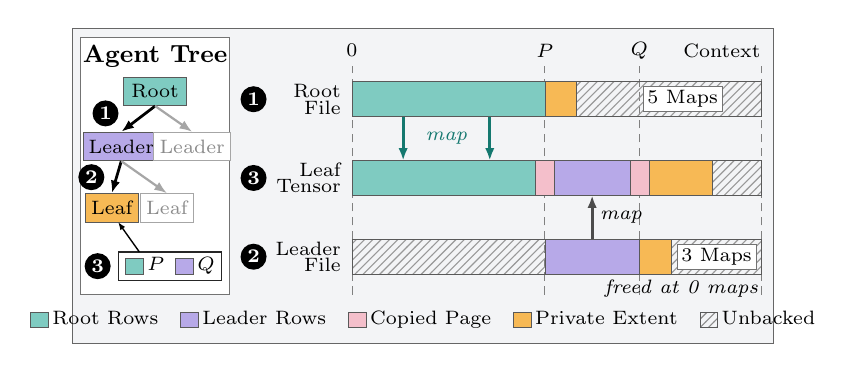
\begin{tikzpicture}[x=1cm, y=1cm, tiny/.style={-{Latex[length=1.0mm]}, line width=0.5pt}]
\draw[layer] (0,0) rectangle (8.9,4.0);

% ---------------- the agent tree ----------------
\draw[sub, fill=white] (0.1,0.62) rectangle (2.0,3.88);
\node[ttl] at (1.05,3.65) {Agent Tree};
\node[blk, fill=sharedc, minimum width=0.8cm] (root) at (1.05,3.2) {Root};
\node[blk, fill=segc, minimum width=0.85cm] (lead) at (0.62,2.5) {Leader};
\node[blk, fill=white, minimum width=0.85cm, text=black!45, draw=black!35] (lead2) at (1.52,2.5) {Leader};
\node[blk, fill=tailc, minimum width=0.6cm] (leaf) at (0.5,1.72) {Leaf};
\node[blk, fill=white, minimum width=0.6cm, text=black!45, draw=black!35] (leaf2) at (1.2,1.72) {Leaf};
% the chain that a leaf receives: every segment with the row at which it ends
\node[comp, minimum width=1.3cm, minimum height=0.36cm, inner ysep=0pt, inner xsep=2pt] (chain) at (1.24,0.98) {\lgdfill{sharedc}\,$P$\enspace\lgdfill{segc}\,$Q$};
\draw[tiny] (0.85,1.16) -- (0.58,1.54);
\draw[arr, line width=1.0pt] (root.south) -- (lead.north);
\draw[arr, black!35] (root.south) -- (lead2.north);
\draw[arr, line width=1.0pt] (lead.south) -- (leaf.north);
\draw[arr, black!35] (lead.south) -- (leaf2.north);
\node[num] at (0.42,2.92) {1};
\node[num] at (0.24,2.11) {2};
\node[num] at (0.32,0.98) {3};

% ---------------- one tensor of the leaf as a chain ----------------
\foreach \x in {3.55,6.0,7.2,8.75} {
  \draw[black!50, line width=0.3pt, densely dashed] (\x,0.62) -- (\x,3.52);
}
\node[tag] at (3.55,3.72) {0};
\node[tag] at (6.0,3.72) {$P$};
\node[tag] at (7.2,3.72) {$Q$};
\node[tag, anchor=east] at (8.78,3.72) {Context};

% the file of the root
\node[tag, anchor=east, align=right] at (3.45,3.1) {Root\\[-2pt]File};
\node[num] at (2.3,3.1) {1};
\node[seg, fill=sharedc, minimum width=2.45cm, minimum height=0.44cm, anchor=west] at (3.55,3.1) {};
\node[seg, fill=tailc, minimum width=0.4cm, minimum height=0.44cm, anchor=west] at (6.0,3.1) {};
\node[free, minimum width=2.35cm, minimum height=0.44cm, anchor=west] at (6.4,3.1) {};

% one tensor of the leaf
\node[tag, anchor=east, align=right] at (3.45,2.1) {Leaf\\[-2pt]Tensor};
\node[num] at (2.3,2.1) {3};
\node[seg, fill=sharedc, minimum width=2.33cm, minimum height=0.44cm, anchor=west] at (3.55,2.1) {};
\node[seg, fill=copyc, minimum width=0.24cm, minimum height=0.44cm, anchor=west] at (5.88,2.1) {};
\node[seg, fill=segc, minimum width=0.96cm, minimum height=0.44cm, anchor=west] at (6.12,2.1) {};
\node[seg, fill=copyc, minimum width=0.24cm, minimum height=0.44cm, anchor=west] at (7.08,2.1) {};
\node[seg, fill=tailc, minimum width=0.8cm, minimum height=0.44cm, anchor=west] at (7.32,2.1) {};
\node[free, minimum width=0.63cm, minimum height=0.44cm, anchor=west] at (8.12,2.1) {};

% the segment file of the leader
\node[tag, anchor=east, align=right] at (3.45,1.1) {Leader\\[-2pt]File};
\node[num] at (2.3,1.1) {2};
\node[free, minimum width=2.45cm, minimum height=0.44cm, anchor=west] at (3.55,1.1) {};
\node[seg, fill=segc, minimum width=1.2cm, minimum height=0.44cm, anchor=west] at (6.0,1.1) {};
\node[seg, fill=tailc, minimum width=0.4cm, minimum height=0.44cm, anchor=west] at (7.2,1.1) {};
\node[free, minimum width=1.15cm, minimum height=0.44cm, anchor=west] at (7.6,1.1) {};

% the same pages
\foreach \x in {4.2,5.3} {
  \draw[arr, roline, line width=1.1pt] (\x,2.88) -- (\x,2.32);
}
\node[note, text=roline] at (4.75,2.6) {map};
\draw[arr, black!70, line width=1.1pt] (6.6,1.32) -- (6.6,1.88);
\node[note, anchor=west] at (6.66,1.6) {map};

% the processes that map each file; its pages remain until the last one leaves
\node[tag, fill=white, draw=black!55, line width=0.3pt, inner sep=1.5pt] at (7.75,3.1) {5 Maps};
\node[tag, fill=white, draw=black!55, line width=0.3pt, inner sep=1.5pt] at (8.18,1.1) {3 Maps};
\node[note, anchor=east] at (8.75,0.7) {freed at 0 maps};

% legend
\node[tag] at (4.45,0.3) {\lgdfill{sharedc}\,Root Rows\quad\lgdfill{segc}\,Leader Rows\quad\lgdfill{copyc}\,Copied Page\quad\lgdfill{tailc}\,Private Extent\quad\lgdhatch\,Unbacked};
\end{tikzpicture}
\end{document}
